%%
%% This is file `./samples/longsample.tex',
%% generated with the docstrip utility.
%%
%% The original source files were:
%%
%% apa7.dtx  (with options: `longsample')
%% ----------------------------------------------------------------------
%% 
%% apa7 - A LaTeX class for formatting documents in compliance with the
%% American Psychological Association's Publication Manual, 7th edition
%% 
%% Copyright (C) 2019 by Daniel A. Weiss <daniel.weiss.led at gmail.com>
%% 
%% This work may be distributed and/or modified under the
%% conditions of the LaTeX Project Public License (LPPL), either
%% version 1.3c of this license or (at your option) any later
%% version.  The latest version of this license is in the file:
%% 
%% http://www.latex-project.org/lppl.txt
%% 
%% Users may freely modify these files without permission, as long as the
%% copyright line and this statement are maintained intact.
%% 
%% This work is not endorsed by, affiliated with, or probably even known
%% by, the American Psychological Association.
%% 
%% ----------------------------------------------------------------------
%% 
\documentclass[man]{apa7}

\usepackage[american]{babel}
\usepackage{nicefrac}
\usepackage{todonotes}
\usepackage{epigraph}
\usepackage{amsfonts, amsmath,amssymb}

\newcommand{\SR}[1]{} %for EJ's bibtex file
\newcommand{\given}{\, | \,}
\newcommand{\EJ}[1]{\todo[inline, color=green]{  #1 }}
\newcommand{\JR}[1]{\todo[inline, color=gray]{  #1 }}
\newcommand{\MK}[1]{\todo[inline, color=red]{  #1 }}

\usepackage{graphicx}
\graphicspath{ {images/} }

\usepackage{csquotes}
\usepackage[style=apa,sortcites=true,sorting=nyt,backend=biber]{biblatex}
\DeclareLanguageMapping{american}{american-apa}
\addbibresource{bibliography.bib}
\addbibresource{referenties.bib}

% \setlength{\parindent}{8ex}

% \usepackage{authblk}

\title{Building Trust in Science Through a Bayesian Perspective on Probability and Uncertainty}
\shorttitle{Building Trust Through a Bayesian Perspective}

\threeauthors{Joshua M. Rosenberg}{Marcus Kubsch}{Eric-Jan Wagenmakers}
\threeaffiliations{University of Tennessee, Knoxville}{IPN - Leibniz Institute for Science and Mathematics Education}{University of Amsterdam}

% \authorsnames[1,2,3]{Joshua M. Rosenberg, Marcus Kubsch, Eric-Jan Wagenmakers}
% \authorsaffiliations{{University of Tennessee, Knoxville},{IPN - Leibniz Institute for Science and Mathematics Education},{University of Amsterdam}}

\leftheader{Weiss}

\abstract{
Uncertainty is ubiquitous in science and this uncertainty takes many forms, but the rhetoric around scientific knowledge and negotiating standards of evidence is often portrayed as immutable. Adding to this problem around the limited recognition of the tentative nature of science, when scientists try to communicate their uncertainty, research has shown us that many—including both learners and experts—struggle to interpret the statistics that are often used to make inferences from scientific data. We argue that a Bayesian approach can offer a different foundation and language around a core but sometimes unsettling tenet and persistent feature, uncertainty. Central to this conceptualization is viewing uncertainty probabilistically, as probabilities can provide a language for expressing the degree of uncertainty in our knowledge in a wide range of domains. In this essay, we (a) briefly introduce Bayes' theorem and wider ideas around Bayesian epistemology, (b) elaborate on the importance of probability and uncertainty in science and science education and review how people learn about these concepts and where they face difficulties, and (c) provide conceptual and practical examples within the JASP statistical software of how Bayes could help to address these issues. We conclude with implications and directions for future research focused around bolstering trust in science outside of classroom settings (for which Bayesian approaches could serve as a crosscutting part of science literacy) and in pre-collegiate science classrooms, where Bayes can provide a coherent approach to engaging in numerous science practices such as arguing from evidence and analyzing and interpreting data in a principled and flexible way.
}

\keywords{APA style, demonstration}

\authornote{
   \addORCIDlink{Joshua M. Rosenberg}{0000-0003-2170-0447}
   \addORCIDlink{Marcus Kubsch}{0000-0001-5497-8336}
   \addORCIDlink{Eric-Jan Wagenmakers}{0000-0003-1596-1034} 
   \\
   Joshua M. Rosenberg and Marcus Kubsch contributed equally to this manuscript.
}

\begin{document}
\maketitle

\setlength{\epigraphwidth}{1.0\textwidth} % set for individual epigraph
\epigraph{It is seen in this essay that the theory of probabilities is at bottom only common sense reduced to calculus; it makes us appreciate with exactitute that which exact minds feel by a sort of instinct without being able ofttimes to give a reason for it . . . we shall see that there is no science more worthy of our meditations, and that no more useful one could be incorporated in the system of public instruction.}{Pierre-Simon Laplace, 1829}
\setlength{\epigraphwidth}{0.4\textwidth} % return to default for the next epigraphs
%\nocite{Laplace18291902} %[p. 196]

Uncertainty is ubiquitous in science and this uncertainty takes many forms. For example, measurement uncertainty is present when there are differences (small or large) in the repeated measures of the same object or phenomenon \parencite{pls03} or when the object that is measured, like a plant, is inherently variable in its characteristics \parencite{pls03}. Another form of uncertainty is its role within explanatory theories, such as those associated with evolution and quantum physics, for which central models take the form of probablistic statements, i.e., uncertainty is a core constituent of these models \parencite{g00}. 

Negotiating these many forms of uncertainty in argumentation—and building toward consensus at the same time that uncertainty is present—is a key part of the scientific process \parencite{t00}. In consequence, some philosophers of science have suggested that science is a process that builds increasingly better models which allows us to make increasingly more accurate predictions about the world  \parencite{g10, g06, n02, r77}.

However, while scientists and philosophers of science may be aware of the uncertainty (and limitations) surrounding scientific knowledge and negotiating standards of evidence interpretation, scientific knowledge is still often portrayed as immutable in educational contexts \parencite{d90}. In consequence, trust in science can erode when scientists individually or collectively change their views, such as during the first phase of the COVID-19 crisis in Germany, when scientists faced serious criticism from politicians and the media for changing their opinion based on new information. A similar tension was present in the United States and around the world regarding potential COVID-19 medication, when initial scientific data and changing interpretations of its utility collided with citizens’ skepticism (and, partisan political views).

Adding to this problem around the limited recognition of the tentative nature of science, when scientists try to communicate their uncertainty, research has shown us that many—including learners and experts alike—struggle to interpret statistics such as confidence intervals or error bars \parencite{gkv04, s07, tk74}. Similarly, difficulties in understanding the language of probability can contribute to a struggle on the part of students when learning about concepts such as evolution of nuclear decay that are modelled in terms of probabilistic statements \parencite{fth17}.

Based on accumulating evidence from cognitive psychology, neuroscience, and education, we build on and extend beyond the science and engineering practice of argumentation the foundational work of science educational \parencite{n11, s07} and statistics education scholars \parencite{a02, b02, h_a20, h_j20,me14, s07} to argue for a \EJ{I'd say ``underused'', because Bayes itself is pretty old and now pretty hip} approach to uncertainty and probability that is currently underrepresented in science education (research). Specifically, we argue that it is helpful to consider uncertainty in terms of a Bayesian epistemological framework to help people to understand uncertainty and probability better and to engage with them in a way that leverages their existing ways of thinking. Central to this conceptualization is viewing uncertainty probabilistically, as probabilities can provide a language for expressing the degree of uncertainty in our knowledge in a wide range of domains \parencite{g12}. In this way, we make this conjecture not only on the merits of Bayes' Theorem as a mathematical or statistical tool, but based on a body of psychological and educational research that shows that such an approach is an intuitive way for people to think about data and evidence in the world \parencite{g12} and in classroom contexts \parencite{ll20, n11, s07, so12, w17}.

The remainder of this paper is structured as follows. First, we will introduce Bayes theorem and wider ideas around Bayesian epistemology. Next, we will elaborate on the importance of probability and uncertainty in science (education) and review how people learn about these concepts and where they face difficulties. Then, we will provide examples of how Bayes could help to address these issues before concluding with implications and directions for future research.

\section{Primer on Bayes Theorem and Bayesian Views of Epistemology}

In essence, Bayes' theorem provides a framework for updating one's beliefs about the world from observations in a way that takes prior knowledge into account in a principled manner. Bayes' theorem (Equation 1) states that at any point in time, our knowledge about the world after making a new observation (i.e., our posterior knowledge) can be obtained by multiplying our prior knowledge with a predictive updating factor (e.g., \cite{RouderMorey2019,WagenmakersEtAl2016CD} ):
\begin{equation*}
        \text{Posterior uncertainty} = \text{Prior uncertainty} \times \text{Predictive updating factor}.
\end{equation*}
Mathematically, this can be expressed as  
\begin{equation}
\label{eq:BayesRule}
        p(\theta \mid \text{data}) = p(\theta) \times \frac{p(\text{data} \mid \theta)}{p(\text{data})},
\end{equation}
where $\theta$ is a hypothesis, proposition, claim, parameter value, or in general any particular account of the world about which we are uncertain. The predictive updating factor consists of two components. First, $p(\text{data} \given \theta)$ is the likelihood, that is, the extent to which the observed data were expected under $\theta$. Second, $p(\text{data})$ is the marginal likelihood, that is, the extent to which the observed data were expected without conditioning on $\theta$. If the observed data are more expected (i.e., better predicted) when conditioning on $\theta$, the predictive updating factor is higher than 1, and $\theta$ becomes more credible. 

To make this more tangible, consider the following example. Suppose an educator is interested in the proportion of students that use Windows or MacOS as their operating system. The proportion of Windows users $\theta$ ranges between 0 and 1. Before you start our Bayesian analysis, you need to quantify your background knowledge -- the relative plausibility of the different values for $\theta$. Given their previous experiences as a teacher, their best guess is that about half of the students use MacOS. They would not be surprised if the proportion of Windows users was between 30\% and 70\% but you would be rather surprised to find either no Windows or exclusive Windows usage. 

This background knowledge motivates the use of the dome-shaped prior distribution shown as the dashed line in Figure~\ref{fig:WindowsMacPriorPosterior}.\footnote{This is the beta$(2,2)$ distribution.} Now suppose you start to collect data by asking students about their operating systems. The first ten observations of Windows (W) and MacOS (M) usage that you make are $\{W, W, M, W, M, W, W, M, W, M\}$: six students use Windows, four use MacOS. 

With these data in hand, we then combine our prior knowledge (i.e., the dome-shaped prior distribution) with the predictive updating factor (assuming a binomial likelihood) and obtain the posterior distribution shown as the solid line in Figure~\ref{fig:WindowsMacPriorPosterior}. The posterior distribution is more peaked than the prior distribution, indicating that the data have sharpened our knowledge about $\theta$. In addition, the posterior distribution is higher than the prior distribution for values of $\theta$ between approximately $.4$ and $.75$: these values of $\theta$ predicted the data relatively well and have therefore gained credibility. In contrast, values of $\theta$ lower than $.4$ and higher than $.75$ predicted the data relatively poorly, which is why they have lost credibility compared to the prior.\footnote{Note that the area under a probability distribution equals 1, so that posterior gains for specific regions of $\theta$ cancel out exactly against posterior losses for the other regions.}  

\begin{figure*}[h]
\begin{center}
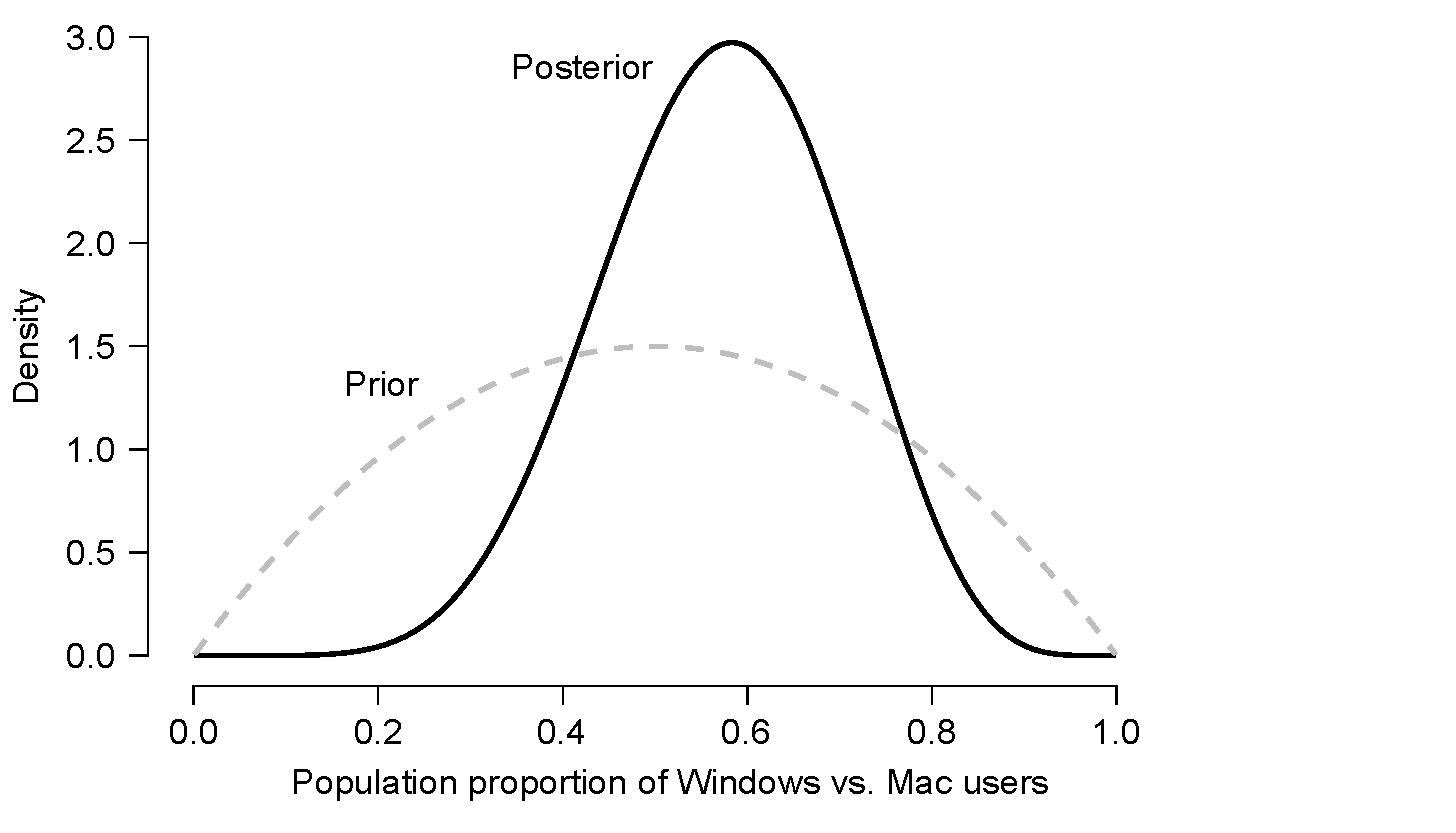
\includegraphics[width = .785\paperwidth]{WindowsMacPriorPosterior.pdf}
\caption{Simple example of Bayesian learning. A dome-shaped prior distribution captures the background knowledge concerning the proportion of students using Windows vs. MacOS. Observing fictitious data from 10 students (six using Windows, four using MacOS) drives a knowledge update that results in a bell-shaped posterior distribution. Figure based on the \emph{Learn Bayes} module in JASP.}
\label{fig:WindowsMacPriorPosterior}
\end{center}
\end{figure*}

Although we have demonstrated this updating process in a single step, it could also be executed sequentially, one student at a time. For instance, the first observation you make is a $W$ and in light of your prior this makes Windows usage a little more likely than MacOS usage. This slight change in knowledge is reflected in the difference between the distributions on the top two lines in Figure~\ref{fig:WindowsMacSequential}; line ``0'' represents the dome-shaped prior distribution and line ``1'' represents the posterior distribution after the first observations. Note that observing a $W$ has nudged the distribution a little to the right. Crucially, the `nudged' posterior distribution after the first observation now takes the role of the prior distribution ready to be updated by our second observation. The second observation is again a $W$, and line ``2'' shows that the resulting posterior distribution is nudged to the right once more. At every stage in the sequential updating process, the posterior distribution based on the observations seen so far becomes the prior distribution for incorporating the information from the next observation. Specifically, the changing distributions in Figure~\ref{fig:WindowsMacSequential} show our knowledge about the world is subject to constant change, by making observations and integrating incoming information with current knowledge using Bayes' theorem. It should be emphasized that although the updating process is conceptually different, the final outcome is identical: the shape of the posterior distribution is unaffected by whether data arrive simultaneously or sequentially.

\begin{figure*}[h]
\begin{center}
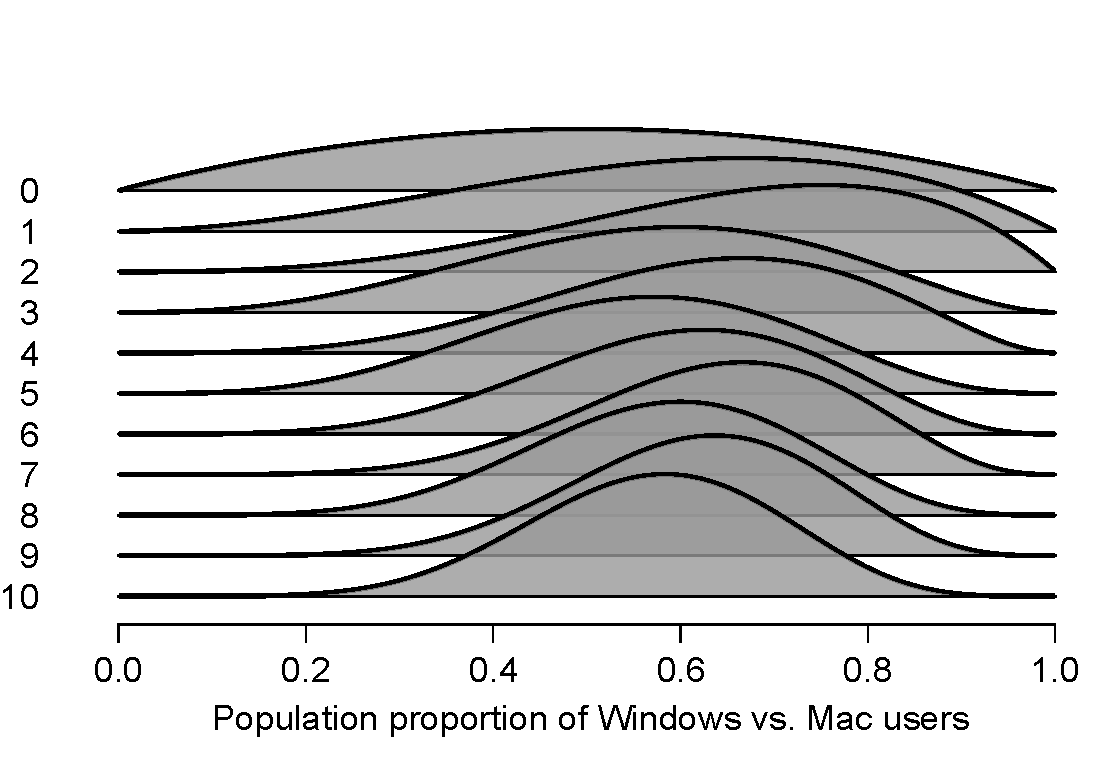
\includegraphics[width = .65\paperwidth]{WindowsMacSequential.pdf}
\caption{Sequential Bayesian learning. A dome-shaped prior distribution (line ``0'') captures the background knowledge concerning the proportion of students using Windows vs. MacOS. Each new observation results in an update to a posterior distribution, which then becomes the prior distribution for the analysis of the next observation. Figure based on the \emph{Learn Bayes} module in JASP.}
\label{fig:WindowsMacSequential}
\end{center}
\end{figure*}

How do the principles from this example translate to students' work with data and evidence -- not only educators? A recent case from physics can serve to illustrate this approach in the context of students' activity in science classrooms. In 2011, physicists reported that they had observed elementary particles moving faster than the speed of light \parencite{b11} - and thus defying Einstein’s theory of relativity. However, instead of celebrating a historic discovery, the scientists started to look for what had gone wrong in their observations. 

How can Bayes’ theorem help to make sense of this? With nearly a century of accumulated evidence that the theory of relativity holds, scientists had a very strong prior belief about the speed of light. To change this belief, extraordinary evidence would have been required. Thus, a single instance of apparently faster-than light elementary particles does not give a likelihood strong enough to change the prior in a meaningful way and in consequence the posterior, the knowledge about the world after making an observation, does not change in a meaningful way. 

Thus, rather than changing their belief about the speed of light, scientists looked for things that could have gone wrong with the measurement. This example shows how a qualitative take on Bayes’ theorem can explain and predict many aspects of how animals \parencite{o13}, people \parencite{tgk06}, and organisations \parencite{kaj12} learn from observations. Recently, advances in computational power and techniques have started the more and more widespread application of this principle in a quantitative way that allows researchers to precisely express their knowledge about the world and then learn from observations. 

Expressed in the Bayesian learning cycle (Figure \ref{fig:The Bayesian Learning Cycle}), a Bayesian reasoning framework allows scientists to integrate the strengths of both, inductive and deductive research approaches, in a formalized way. Further, when specifying the prior, scientists openly and explicitly need to describe the (un)certainty in the current state of knowledge and the posterior captures how the data has changed the knowledge and the (un)certainty in that knowledge. Thus, Bayesian reasoning is, at least in principle, open and transparent by design.

\begin{figure*}[h]
\begin{center}
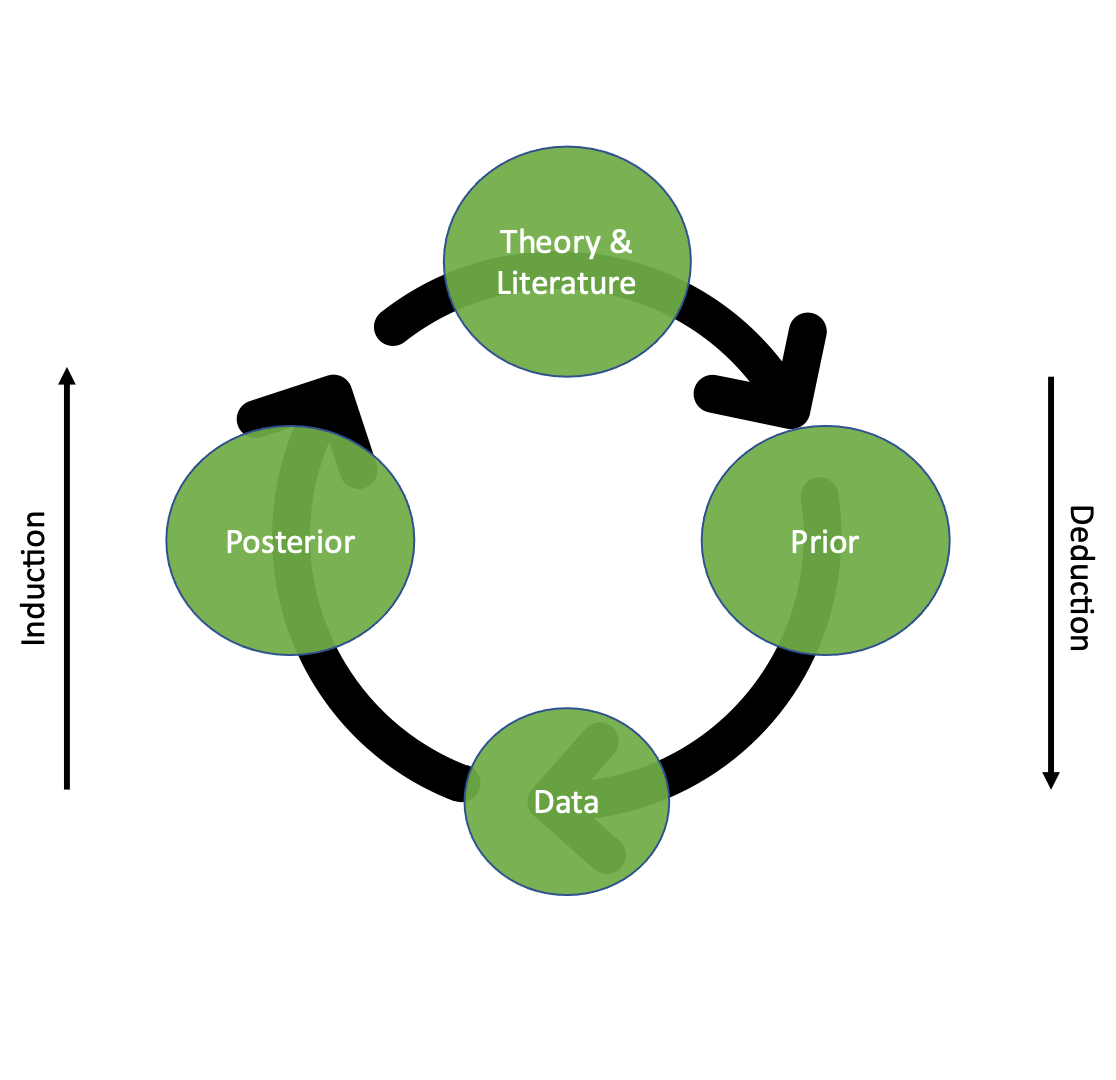
\includegraphics[width = .65\paperwidth]{learning.png}
\caption{The Bayesian Learning cycle}
\label{fig:The Bayesian Learning Cycle}
\end{center}
\end{figure*}

Having introduced Bayes theorem and an application of Bayes theorem as a cycle through which individuals can learn, we describe the role of uncertainty in science, with a focus on the role of probability.

\section{Uncertainty in Science and the Role of Probability}

Probability and uncertainty are ubiquitous in science—in scientific methodologies, the scientific concepts, or in how science is communicated \textcite{gsoobmc17}. The practice of science often begins with measurement, and with measurement comes measurement error, which has a random component. This random component arises from random variations in the measurement process and limits the certainty that one can have in the measurements. Reducing that measurement error has been critical for many discoveries in science, such as in sorting out the periodic table as we know it today \textcite{fco15}. However, deciding on adequate statistical procedures to determine measurement uncertainty regularly sparks debate, e.g., the recent study on the relationship between SARS-CoV-2 viral load and patient age by \textcite{jmvbzhd20} was heavily debated in the scientific community \parencite{frick_peer-review_2020}.

Probability and uncertainty are not only key concepts in science practices such as analyzing and interpreting data, but also part of the scientific concepts themselves. One example is Heisenberg’s uncertainty principle or quantum mechanics more generally \textcite{feynman1951operator}. In quantum mechanics, confidence in measurement is limited not only by measurement error but in principle—even in the perfect experimental setup there is no deterministic outcome. Instead, one has to calculate the probability of each possible outcome using the Born rule. To this day, there is an ongoing argument among physicists and philosophers about how to interpret probability and the puzzling quantum mechanical phenomena such as quantum tunnelling  \textcite{c19}. Another example of how probability and uncertainty are central to learning scientific concepts is  evolution  \textcite{fsnh19}. Evolution is modelled as a probabilistic process as the emergence of new variations (e.g., through mutations) can only be described probabilistically. Further, the continued survival of these variations is governed by phenomena such as natural selection or random drift which also escape a deterministic description and are thus modelled probabilistically.\EJ{I agree that we can only describe the process probabilistically. But that does not mean it \emph{is} probabilistic.} \MK{tried to address this comment as well.} Similar to within quantum physics, how to interpret this probability has also sparked debate among researchers  \textcite{m16}.
Given that probability and uncertainty spark debate among scientists, it is perhaps unsurprising that misinterpretations happen when scientists in the natural and engineering sciences communicate about their findings with their peers or the public \parencite[]{gkv04, c14, mg17}. For example, error bars in the form of confidence intervals are routinely interpreted as distributions that assign higher probability to the center of the interval \parencite{kl18} or \emph{p}-values are interpreted as effect sizes \parencite{gc17, n14} (although p-values describe how (in)compatible a set of data is with a set of assumptions. In sum, misinterpretations of statements about probability and uncertainty are common across the range of modes in which scientists communicate about their work.

\section{Uncertainty in Science Education}

Given the above-noted roles of probability in scientific concepts and theories, it is unsurprising that educational researchers have documented how students learn about probability. As one example, probability and chance events play an important role in the life sciences \parencite{g03, gk08}, particularly in evolutionary processes and learning about them \parencite{th17}. Recently, \textcite{fsnh19} investigated the relation between statistical reasoning and acceptance and knowledge about evolution in a large sample of nearly 500 university students in the US. They found that students’ statistical reasoning capabilities are a strong predictor of both acceptance of evolution and knowledge about evolution. Thus, this study suggests (but does not directly show) that instructional strategies for supporting students’ statistical reasoning could improve their learning about specific evolutionary concepts.

In the physical sciences, students' struggles with the probabilistic nature of quantum physics \parencite{br02} and nuclear decay \parencite{smmv17} are known, but the underlying reasons and mechanisms remain less researched than in evolution. Research into students’ misconceptions inspired by conceptual change research has started to address this gap \parencite{ms15, alra14, st09}. Findings seem to mirror the position of \textcite{bgv94} in that the concepts of probability are taught too abstractly and in a way that does not build upon and connect with the ideas that students’ already hold, the experiences that students make, and the language that students use. Thus, these studies affirm students' struggles with scientific concepts that are probabilistic but hint at the underlying issue being foundational, conceptual struggles with ideas about probability not limited to science learning. Indeed, the language and representations used to communicate probability and uncertainty independent of specific scientific content domains or scientific practices are also known to present difficulties to learners. The work of \textcite{tk74} points to a whole range of biases that the language in which statements about probability and uncertainty are framed can elicit. A prominent example is the neglect of base rate information in the (timely) context of medical testing, that is, the probability of having a medical condition on the basis of a positive test result is often hugely overestimated because information about the base rate of people affected from the condition is neglected \parencite{kahneman_thinking_2012}.

More recent work by Gigerenzer and colleagues has provided important insights into the underlying mechanisms for the occurrence of these biases \parencite{gh95, jkg18}. Their research suggests that the biases are at least partly the result of information about probability and uncertainty being provided in a way that is incompatible with the heuristics that people develop from their everyday experiences. Based on this assumption, \textcite{jkg18} were able to demonstrate that students judge probability significantly better, when language is adopted that better aligns with the heuristics that most learners develop from their everyday experiences. In sum, it seems feasible to change representations of probability and uncertainty so that they better align with ideas and heuristics that learners hold so that these support instead of inhibit learning. 

\section{How Learners and People Make Sense of Data in Light of Uncertainty}

Recent work in cognitive and psychological science on how children learn argues that children understand and learn about the world through the intuitive application of Bayesian ideas \parencite{g12, tgk06, tgk06}. This idea has led current research to conceptualize human learning in terms of Bayesian probabilistic models of learning. In other words, people (and children) may view (or come to view) the world probabilistically, and in ways that happen to align with Bayesian interpretations of probability.

This view of how children learn from data has become especially prominent in developmental science and is successfully applied there \parencite{gt07, gw12}. One might assume that there has been a ready application of these ideas about how children think about the world in a Bayesian way to education. Developmentalists have pointed to the potential and opportunity here. \textcite{g12} wrote that the use of Bayesian methods to understand child development can serve as “a scientific foundation for a long tradition on ‘inquiry-based’ science education,” that “could lead us to much more specific and scientifically supported proposals for education” (p. 1627).  

Despite arguments for integrating developmental and educational research, it has largely not been the case that—with respect to advances in Bayesian methods—“science itself could help turn young children’s natural curiosity and brilliance into better science teaching and learning” \textcite[p. 1627]{g12}, as some science education scholars have bemoaned \parencite{ls15}). Indeed, scholars have argued that it is often obsolete applications of Piaget’s ideas \textcite{pi69} that represent the greatest contribution of developmental ideas to education \textcite{ls07}. We argue that this is still largely the case in the present, despite advances in both developmental research as well as statistical methodology related to Bayesian ideas—and that it is time to start exploring how bringing out the inherent Bayesian ways of thinking in education may provide support for learners’ efforts to make sense of the world.

Related science education research emphasizes the role of prior knowledge that students bring with them to the analysis of data and how that prior knowledge impacts the inferences they make about data. For example, \textcite{mkm07} summarized findings across a number of studies showing that when elementary grade students reasoned with data in a context about which they had strong and valid prior understandings that informed their interpretation of data (about force and motion in the context of ramps), and they were able to explain sources of error in the data \parencite{mk03}, but when the data was in a context they did not understand well, they struggled to distinguish between random variation due to sources of error and sources of variation due to something that was causing a difference in the data (generated by measuring the motion of pendulums). Later design- and laboratory-based research has shown that students can develop an understanding of scientific ideas through the analysis of data \parencite{ls04,mkk17}.

Laboratory-based research, especially, has examined how learners’ prior understanding may have a bearing on how they make sense of how likely different outcomes are \parencite{kd88, mkm07, ssc07}. While these studies focused on how students’ prior ideas and data interact, Bayesian frameworks were not used to formalize this process of integrating data in light of prior beliefs about scientific phenomena. In short, this work aligns closely with the Bayesian models of how children learn from data described by \textcite{g12}, but this research does not explicitly interpret their findings in light of these ideas about how children learn from data in a Bayesian way.

Overall, developmental and psychological research into Bayesian models of cognition supports and bolsters efforts in science education to design instruction based around eliciting and understanding students’ ideas \parencite{gb16, hbavb20, wtbs12}. There is an opportunity to use Bayesian ideas as a framework for formalizing these ideas about how prior ideas affect students’ reasoning about data and how teachers can leverage students’ ideas to design instruction, yet Bayes has mostly been absent from research in science education.
After having reviewed how people learn about probability and uncertainty and where they face difficulties, we want to present how Bayes could be part of a solution. First, we will make the case how Bayes could support science literacy at large before delving into more concrete topics.

\section{Bayes and Science Literacy}

\subsection{Overview of Bayes and Science Literacy}

Having described the role of probability and uncertainty in science and science education, we now describe what these Bayesian ideas can mean for science literacy. We see two primary ways in which Bayesian methods can enhance science literacy, or a range of capabilities that people may possess which have value (individually or collectively) to them \parencite{council2016science}. These capabilities range from foundational literacies, including numeracy and textual literacy (what is most thought of concerning literacy in common parlance), content knowledge, and epistemic knowledge and other ways of thinking and habits of mind \parencite{council2016science}. One way that Bayesian ideas can inform discussions of science literacy is to provide individuals with a technique for combining their prior understanding with new evidence. Along this line, Bayes and the Bayesian learning cycle more specifically can provide a conceptual tool for people to combine their understanding with new evidence (and data) in a rigorous and coherent way, as we discuss next. 

The history of science is, in many ways, a story of established ideas being built upon or supplanted \parencite{fara2010science}, and the contemporary emphasis on viewing science as a practice was sparked by \textcite{k62} historical-epistemological account on what this suggests about the nature and philosophy of science \parencite{g09}. Yet, our ways of interpreting scientific evidence do rarely recognize this, perhaps for good reason: Most of the time, new data or information do not contradict foundational scientific ideas \parencite{k62}. The same phenomenon, though, is present on a more micro-level: While scientists may be familiar with the data they collect not eliding with ideas that are a part of the scientific consensus, in media and the public discourse scientific ideas are often presented as fixed and certain—even in cases for which consensus has not been reached \parencite{c87}

These historical and philosophical ideas align with a Bayesian perspective on science literacy. Established scientific ideas can be considered to be those that individual people - psychologically - should be more confident about, whereas newer ideas, or data suggesting new ideas, can be weighted less. In this way, Bayes can provide a simple heuristic for people to evaluate new information or evidence; by asking the question of how informative is the evidence in light of the prior. Thus, individuals possess a tool, one that is non-dichotomous, in that the evidence is not true or false, and also probabilistic, in that what individuals can think, going forward, is about the extent to which a particular belief has merit and is informative.

A concrete example can help to illustrate how a Bayesian perspective on a topic relevant to science literacy may offer a different way forward. Consider a salient topic, medical vaccines for diseases, such as Polio and the disease caused by the coronavirus SARS-CoV-2, COVID-19. Most evidence suggests that vaccines have been safe, historically, and are generally safe, at present (Centers for Disease Control and Prevention, 2021). Nevertheless, they are not perfectly safe, as unlikely, adverse outcomes do happen, and it is possible that there are adverse side effects from some vaccines that research has not yet revealed. In light of this evidence, consider the development of a new vaccine, such as those available at the time of this writing for COVID-19. Some use long-established methods of vaccine development (namely, deactivating SARS-CoV-2 particles but retaining cell signalling proteins to which humans develop an immune response—and, after, a degree of immunity) and injecting these deactivated virus particles into people), whereas others use a new mechanism (namely, injecting messenger RNA into people; this messenger RNA is then transcribed by cells in people’s bodies to produce a particular protein common to SARS-CoV-2 particles, which human’s bodies than learn to recognize to develop immunity.

How should we consider evidence about the vaccines? Prior to any data from medical clinical trials, it would be reasonable to consider these vaccines to probably be safe in light of the safety of other vaccines (and on the basis of similarities in their mechanisms of action), but to have a strong degree of caution about how safe they are. After initial trials were completed, the degree of safety that individuals associate with these vaccines—in light of the prior and the limited evidence—could increase, but still not be near the level of safety that many would consider acceptable. Following the completion of clinical trials that show minimal side effects (holding aside their efficacy), one’s estimates of the safety of these vaccines could increase by a substantial amount, but concerns could still remain, particularly for messenger RNA vaccines, which are newer, and may, plausibly, have unintended side effects.

\subsection{Strategies for Supporting Science Literacy}

What is the result of this entire process of weighting new evidence in light of a generic prior that we discussed above? We argue that there are three ways that Bayesian methods could support science literacy. 

The famous French astronomer and mathematician Laplace argued that Bayes' rule quantifies how rational observers ought to change their opinion in light of new evidence; in this sense, Laplace believed that Bayes' rule was \emph{common sense expressed in numbers}. We now showcase several insights that follow directly from Bayes' rule. In our earlier exposition of Bayes' rule we already emphasized the idea that hypotheses gain credibility when they predict the data well, and lose credibility when they predict new data poorly \parencite{WagenmakersEtAl2016CD}. This idea generalizes what the mathematician Polya termed the ``Fundamental Inductive Pattern'':
\begin{quotation}
``This inductive pattern says nothing surprising. On the contrary, it expresses a belief which no reasonable person seems to doubt: \emph{The verification of a consequence renders a conjecture more credible}. With a little attention, we can observe countless reasonings in everyday life, in the law courts, in science, etc., which appear to confirm to our pattern.'' \parencite[pp. 4-5]{Polya1954Vol2}
\end{quotation}

The rule from Equation~\ref{eq:BayesRule} includes the constant term $p(\text{data})$, which does not involve $\theta$. Hence, we can also write Bayes' rule as:
\begin{equation}
\label{eq:BayesRulePropto}
p(\theta \mid \text{data}) \propto  p(\text{data} \mid \theta) \times p(\theta),
\end{equation}
where `$\propto$' stands for `is proportional to'. Thus, Bayes' rule states that our posterior knowledge $p(\theta \given \text{data})$ is proportional to the likelihood $p(\text{data} \given \theta)$ (i.e., predictive adequacy, unsurprise, or the extent to which the observed data are expected given $\theta$) multiplied with our prior knowledge $p(\theta)$.

Equation~\ref{eq:BayesRulePropto} emphasizes the fact that the posterior uncertainty about $\theta$ is a \emph{compromise} between our prior uncertainty about $\theta$ and the predictive performance of $\theta$. But the posterior uncertainty after having observing the first datum becomes the prior uncertainty for the to-be-observed second datum (cf. Figure~\ref{fig:WindowsMacSequential}). Consequently, after having observed the second datum, the posterior uncertainty represents a compromise of a compromise. As the data accumulate, the posterior uncertainty is more and more determined by predictive performance, and the impact of the initial uncertainty about $\theta$ is increasingly watered down: `the data overwhelm the prior' \parencite{WrinchJeffreys1919}.

This implies that a constant stream of accumulating data ought to bring any two rational people into an arbitrarily close agreement, no matter how divergent their opinions may have been at the outset. There are two important caveats here. First and foremost, the data only overwhelm the prior if that prior is neither 0 (denoting an impossibility) nor 1 (denoting absolute certainty). If you already know for certain that a hypothesis is true or false, then you cannot adjust your opinion in light of the data: your initial opinion will be your final opinion, no matter what the data may indicate. Philosophically, adopting such priors is a dangerous practice; for instance, in antiquity the adage of the \emph{New Academy} --a school of skeptics headed by Carneades-- was ``never assert absolutely''. In modern times, Lindley popularized this idea in statistics and coined it ``Cromwell's rule'':
\begin{quotation}
``Consequently, an uncertain event of zero probability remains so whatever information is provided. In other words, if a decision-maker thinks something cannot be true and interprets this to mean it has zero probability, he will never be influenced by \emph{any} data, which is surely absurd. So leave a little probability for the moon being made of green cheese; it can be as small as 1 in a million, but have it there since otherwise an army of astronauts returning with samples of the said cheese will leave you unmoved. A probability of one is equally dangerous because then the probability of $\bar{E}$ will be zero. So never believe in anything absolutely, leave some room for doubt: as Oliver Cromwell told the Church of Scotland, `I beseech you, in the bowels of Christ, think it possible you may be mistaken'.'' \parencite[p. 104]{Lindley1985} 
\end{quotation}

The second caveat is that, in real life, the data are sometimes relatively slow to overwhelm the prior, as people can be reluctant to change their beliefs (for a Bayesian model see \cite{Gershman2019}). A more extreme case is \emph{belief polarization}: confronted with the same stream of information, two people who hold different opinions may drift further apart instead of moving closer together (but see \cite{Anglin2019}). This appears irrational, but several Bayesian accounts have been offered to explain the phenomenon (e.g., \cite{CookLewandowsky2016,JernEtAl2014}).

Now consider two specific values for $\theta$, $\theta_1$ and $\theta_2$. We can use Bayes' rule to obtain the posterior probability for each one:
\begin{align}
p(\theta_1 \mid \text{data})& =  \frac{p(\text{data} \mid \theta_1) \times p(\theta_1)}{p(\text{data})}\\
p(\theta_2 \mid \text{data})& =  \frac{p(\text{data} \mid \theta_2) \times p(\theta_2)}{p(\text{data})}.
\end{align}
When we divide the posterior probabilities the common term $p(\text{data})$ drop out and we have:
\begin{equation}
    \frac{p(\theta_1 \mid \text{data})}{p(\theta_2 \mid \text{data})} = \frac{p(\theta_1)}{p(\theta_2)} \, \times \, \frac{p(\text{data} \mid \theta_1)}{p(\text{data} \mid \theta_2)}.
\end{equation}
We replace $\theta_2$ with $\mathcal{H}_1$ (i.e., the alternative hypothesis, in which a test-relevant parameter $\xi$ is free to vary) and $\theta_1$ with $\mathcal{H}_0$ (i.e., the null hypothesis in which $\xi$ takes on a fixed value, for instance $\xi=0$):
\begin{equation}
    \frac{p(\mathcal{H}_1 \mid \text{data})}{p(\mathcal{H}_0 \mid \text{data})} = \frac{p(\mathcal{H}_1)}{p(\mathcal{H}_0)} \, \times \, \frac{p(\text{data} \mid \mathcal{H}_1)}{p(\text{data} \mid \mathcal{H}_0)}.
\end{equation}
This way of writing Bayes' rule highlights that extraordinary claims require extraordinary evidence -- if a particular hypothesis $\mathcal{H}_1$ is extremely unlikely a priori, the prior odds $\frac{p(\mathcal{H}_1)}{p(\mathcal{H}_0)}$ are stacked against it, and in order for the posterior odds to favor $\mathcal{H}_1$ the support from the data (i.e, the degree to which $\mathcal{H}_1$ outpredicts $\mathcal{H}_0$) needs to be overwhelmingly strong.   

Bayes' rule can also be shown to embody the \emph{principle of parsimony}: the rule implicitly contains a preference for the simplest model that explains the data well. To see this, consider a coin taken from a magician's coffin, and let parameter $\xi$ indicate the chance that the coin lands heads on any throw. The null hypothesis holds that the coin is fair, $\mathcal{H}_0: \xi = \nicefrac{1}{2}$. The alternative hypothesis that we entertain here specifies that the coin may be double-tails, fair, or double-heads, $\mathcal{H}_1: \xi \in \{0, \nicefrac{1}{2}, 1\}$, with each of the three options deemed equally likely a priori. 

The coin is tossed and we observe heads. The probability of this datum is \nicefrac{1}{2} under $\mathcal{H}_0$; under $\mathcal{H}_1$, it is $p(\text{heads} \given \xi=0) \cdot p(\xi=0 \given \mathcal{H}_1) + p(\text{heads} \given \xi=\nicefrac{1}{2}) \cdot p(\xi=\nicefrac{1}{2} \given \mathcal{H}_1) + p(\text{heads} \given \xi=1) \cdot p(\xi=1 \given \mathcal{H}_1) = 0 \cdot \nicefrac{1}{3}  + \nicefrac{1}{2} \cdot \nicefrac{1}{3} + 1 \cdot \nicefrac{1}{3} = \nicefrac{1}{2}$. So the datum is equally likely under $\mathcal{H}_0$ and $\mathcal{H}_1$: both models receive an equal amount of support. This means the first outcome does not change our conviction concerning $\mathcal{H}_0$ versus $\mathcal{H}_1$. The datum did, however, change our beliefs about $\xi$ under $\mathcal{H}_1$. Specifically, we now know that $\xi$ cannot be 0; moreover, the datum was twice as likely under $\xi=1$ as under $\xi = \nicefrac{1}{2}$, so that our posterior distribution for $\xi$ under $\mathcal{H}_1$ is now $p(\xi = \nicefrac{1}{2}) = \nicefrac{1}{3}, p(\xi = 1) = \nicefrac{2}{3}$. 

The coin is tossed a second time and it lands tails. Under $\mathcal{H}_0$, the probability of this happening is again $\nicefrac{1}{2}$, so the total probability for the data sequence $\{\text{heads}, \text{tails}\}$ under $\mathcal{H}_0$ equals $\nicefrac{1}{2} \cdot \nicefrac{1}{2} = \nicefrac{1}{4}$. Under $\mathcal{H}_1$, the probability of the second toss landing heads is computed under the posterior distribution obtained after the first toss, and this yields: $p(\text{tails} \given \xi = \nicefrac{1}{2}) \cdot p(\xi=\nicefrac{1}{2} \given \mathcal{H}_1) + p(\text{tails} \given \xi = 1) \cdot p(\xi=1 \given \mathcal{H}_1) = \nicefrac{1}{2} \cdot \nicefrac{1}{3} + 0 \cdot \nicefrac{2}{3} = \nicefrac{1}{6}$. The total probability for the data sequence $\{\text{heads}, \text{tails}\}$ under $\mathcal{H}_1$ equals $\nicefrac{1}{2} \cdot \nicefrac{1}{6} = \nicefrac{1}{12}$. This means that the observed data provided $(\nicefrac{1}{4}) / (\nicefrac{1}{12}) = 3$ times more support for $\mathcal{H}_0$ than for $\mathcal{H}_1$. This happens because $\mathcal{H}_1$ spreads out its predictions, hedging its bets. In contrast, the simple model $\mathcal{H}_0$ made a precise prediction. 

Instead of learning about the predictive performance of $\mathcal{H}_0$ and $\mathcal{H}_1$ one observation at a time, we could also have considered the probability that the models assign to the entire sequence $\{\text{heads}, \text{tails}\}$. Under $\mathcal{H}_0$ we again have $\nicefrac{1}{2} \cdot \nicefrac{1}{2} = \nicefrac{1}{4}$. Under $\mathcal{H}_1$, we notice that the data falsify both $\xi=0$ and $\xi=1$. This leaves $\xi=\nicefrac{1}{2}$, which suggests the same answer as under $\mathcal{H}_0$, that is $\nicefrac{1}{2} \cdot \nicefrac{1}{2} = \nicefrac{1}{4}$. However, we need to multiply this probability with $\nicefrac{1}{3}$, the prior probability that $\xi=\nicefrac{1}{2}$. This is the penalty for complexity that $\mathcal{H}_1$ pays for entertaining three different values of $\xi$ from the outset. 

Thus, Bayes rule includes a automatic ``Ockham's razor'' \parencite{Jeffreys1939,JefferysBerger1992} in the sense that daring predictions are rewarded when they come true.

Finally, we can also write Bayes' rule as follows:
\begin{equation}
\begin{split}
    p(\mathcal{H}_1 \mid \text{data})& = \frac{p(\text{data} \mid \mathcal{H}_1) p(\mathcal{H}_1)}{p(\text{data})}\\
    & = \frac{p(\text{data} \mid \mathcal{H}_1) p(\mathcal{H}_1)}{p(\text{data} \mid \mathcal{H}_1) p(\mathcal{H}_1) + p(\text{data} \mid \mathcal{H}_0) p(\mathcal{H}_0)}.
\end{split}
\end{equation}
This equation shows that the posterior plausibility is dictated by the predictive performance for $\mathcal{H}_1$ and $\mathcal{H}_0$, weighted by the prior plausibility of each hypothesis. In other words, ``The Bayesian world is a comparative world in which there are no absolutes.'' \parencite[p. 308]{Lindley2000}. This is in stark contrast to $p$-value statistical hypothesis testing, in which a statistical model (the null hypothesis) is judged in isolation. 

Thus, in summary, the result of applying Bayes rule is a non-binary inference, one that doesn't speak to whether or not the vaccine is safe, but to what degree it is safe, doing so with a language of probability and uncertainty. Though a small difference, discussing the safety of vaccines on these terms can provide a more solid foundation for principled disagreements and arguments. In addition, Bayes provides a heuristic and a language for engaging with uncertainty in a science literacy context in a principled way that is in-line with how most of us likely already interpret data. Specifically Bayes provides people with a way to talk about weighing between ideas and their prior beliefs and new information and data. In short, Bayes gives people a chance to deal with uncertainty in a principled but accessible way.

\section{Bayes and Science Education}

\subsection{Overview of Bayes and Science Education}

Research on the role of Bayes in science education has mostly been carried out in the context of undergraduate statistics education, in which there have been a number of calls to action \parencite{gpkpwc18, h_a20}, examples and design options \parencite{a02, b02,g08, w17, h_j} and debate \parencite{jrhrr20} over how to advance the place of Bayesian methods in undergraduate statistics and data science degree programs. The accessibility of Bayesian methods in undergraduate classes is the result of advances in the necessary (for many uses) computer power \parencite{gpkpwc18} as well as the availability of tools that facilitate Bayesian analysis, especially for newcomers \parencite{ah20} .As evidenced by the recent special issue of the \emph{Journal of Statistics Education} of which several of the above-referenced articles are part, the pedagogy of Bayesian statistics is an active area of research in statistics education at the undergraduate level.

There is little research outside of statistics education in the broader science education community. Two publications merit mention though. The work of \textcite{so12} and \textcite{n11} both applied Bayesian perspectives to the science practice of argumentation. Szu and Osborne presented the case for how and why Bayes Theorem can apply to research and practice on scientific reasoning, broadly, and argumentation, particularly. This paper represents the most comprehensive account of the relevance of Bayesian methods for science education. Szu and Osborne argue that Bayes is useful as both a formal mathematical tool, and a conceptual one; indeed, they write that considering the degrees of certainty in beliefs that individual students hold—different from applications of Bayes Theorem that follow more or less deterministically from ``external, objectively probabilistic systems'' (p. 61)—is ``the key leap that characterizes the debate about the value of Bayesian inference as a model of scientific reasoning'' (p. 61). In this way, Szu and Osborne argue that the greatest use of Bayes theorem in science classrooms is as a model of informal scientific reasoning, aligning with similar (informal) approaches to inference within the statistics education research community \parencite{batanero2016research, mr18}. They offer some research-related backing for the use of Bayes Theorem (e.g., noting how conceptual change research, particularly, and constructivist research, broadly, can both be explained coherently within a Bayesian approach) as well as some practical, instructional recommendations, some of which we detail later in this section.

\textcite{n11} work on Bayesian approaches to argumentation complement the work of Szu and Osborne in that Nussbaum describes both an application of Bayesian methods in K-12 classroom contexts and ideas about how Bayesian methods can serve as an analytic framework for students’ argumentation. Concerning the latter, Nussbaum describes how the social issue of raising taxes to provide resources to homeless individuals was a rich context for students to engage in forms of Bayesian reasoning. In this application, Nussbaum describes how the prior and likelihood could be obtained from empirical evidence—in this way, illustrating what \textcite{so12} characterize as the more externally objective use of Bayes Theorem—and how the estimates that result from applying Bayes theorem led students to re-evaluate their initial arguments. 

In summary, the work of \textcite{so12} and \textcite{n11} begin to apply Bayesian ideas to science education and other relevant classroom contexts, making Bayesian ideas more vivid in the process. Curiously, no work has applied Bayesian methods to another science practice, that of analyzing and interpreting data; one for which Bayesian methods have clear conceptual applicability and utility, but one for which the absence of suitable tools may provide to be a barrier. In this way, Bayesian methods could serve as a cross-cutting concept \parencite{nrc12} that unites the practice of argumentation with analyzing and interpreting data, and using mathematics and computational thinking.

\subsection{Strategies for Supporting Science Education}

Bayesian methods clearly have some utility in science education, even if that utility is under-realized at present. Next, we present some of the specific ways Bayesian methods could enhance science education—and could do so in a way that makes Bayes more tractable.

First, we should consider ``unplugged'' versions of Bayesian analyses, akin to how computer science education scholars have emphasized that computational thinking does not necessarily require the use of a computer (Yadav et al., 2018). These could interface with the science and engineering practice of modeling; could students use diagrammatic models in conjunction with Bayesian “heuristics” to revise their models in a similar manner to how this practice can unfold in classrooms \parencite{schwarz2009developing}. 

Another advance should be to build out curricular strategies, elaborating on the ideas of \textcite{so12} and \textcite{n11}. At a high-level, Szu and Osborne write that in order to reason about data in light of their initial beliefs (and to construct a kind of informal likelihood statistic), students “need to see judgments about data and evidence being an assessment not only of the probability of the hypothesis being correct but also of it being wrong” (p. 67). Filling in more details, speaking from both the perspective of a researcher (of argumentation) and an educator (or, a designer of classroom activities), Nussbaum summarizes that using Bayes “forces one to (a) think about an issue from different perspectives, (b) reflect on one’s range of certainty and uncertainty, and (c) conduct a simple com- puter simulation (e.g., calculating the product) that integrates various facets of the issue together and affords further reflection” (p. 99). 

These are helpful suggestions, and they complement finer-grained instructional techniques, especially those around how students can reason about uncertainty probabilistically. Particularly, \textcite{bkbm18} for instance, suggest replacing probabilities with natural frequencies in alignment with a great deal of work on how humans understand probability) \parencite{gh95} as well as using and interpreting tree diagrams to depict natural frequencies. \textcite{me14}—building on much earlier experimental work by \textcite{wason1971natural}—provide a simple example of how even fourth graders, with the right tools to represent probabilities, can support students to transition from logical to probabilistic reasoning. These could also support the aim of developing unplugged versions of Bayesian analyses. 

Third, we should, of course, consider teachers and how teachers can (or already) support students to reason about uncertainty, and, possibly, to use Bayesian ideas. While some scholars have contributed foundational work demonstrating how this uncertainty can be productive as a part of teaching practice \parencite{manz2018supporting}, a broad and formal perspective on how uncertainty can be approached in science education is needed. There is the need to explore the potential of a principled approach to uncertainty, one that may be intuitive to learners and useful to teachers, but is as yet under-represented in the science education literature. If learners and people better understand uncertainty, they can better understand the scientific process which helps to build trust in science. Further, a better understanding of uncertainty can help to learn about scientific--and other--concepts where probability plays a key role; it may be that learning about how Bayes rule can be used in legal or medical contexts could impress upon students the cross-cutting nature of probability and uncertainty. This is especially helpful in light of the teacher's practice of noticing and responding to students' ideas and the process through which students change their understanding.

Finally, recently developed tools, particularly the JASP statistical software, may be helpful. JASP allows for both conventional frequentist as well as Bayesian versions of commonly used statistical tests, such as t-tests and regression analyses. There are a number of accessible guides available for specifying Bayesian versions of analyses \parencite{v20, wagenmakers2018bayesian}, and there is a great potential in building particular examples within JASP (that are aligned to science education curricular standards) that could support science educators to have greater access to the power of Bayesian methods in their classrooms. Another possibly useful tool could be Bayesian networks (see Bayes Box; Bayes Box, 2021), which could be used to model complex system in a way that is similar to other tools used in science education for modeling complex systems, such as \textcite{20}.

\section{Summary and Conclusion}

While some educational researchers may state that such theoretical, abstract ideas about the philosophical and statistical underpinnings of working with data are irrelevant to how students work with data, we make the case, here, that these ideas can inform instructional practice, assessments, and the design of activities that involve students in working with data, especially given some of the clear problems that have been articulated around the present frequentist Null Hypothesis Statistical Testing (NHST)-based approaches \parencite{c14, gkv04}.

Science education researchers may note that these ideas are conceptually-focused, rather than aligning with the present emphasis in science education upon engaging students in science and engineering practice in order to make sense of core ideas and to engage with cross-cutting concepts \parencite{nrc12}. We argue that Bayes is unique in that it, perhaps akin to a cross-cutting concept in the sense of a style of reasoning \parencite{so12, ork18} that blends conceptual ideas with practices. Bayes is both a philosophical and psychological perspective on how to learn from data as well as a statistical framework. Indeed, a key potential benefit of Bayes may be that it provides a framework for helping students to transition from their conceptual understanding of scientific ideas to quantitatively analyzing data.

In this paper, we have introduced Bayes as a powerful way of conceptualizing probability and uncertainty. These are two concepts that are ubiquitous in the learning, doing, and communicating of science and therefore critical aspects of science literacy \parencite{}. However, probability and uncertainty are also infamously challenging concepts—for experts and laypersons alike \parencite{gkv04, s07, tk74}. Thus, it is not surprising when the public misinterprets statements about probability and uncertainty but the consequences may be dire when trust in science is eroded, and, sadly, examples of this are plentiful during current the COVID-19, e.g., the efficiency of masks in preventing the spread of COVID and the efficiency of the AstraZeneca vaccine were strongly questioned, delaying efforts to comb at the pandemic. The public, however, can hardly be blamed for this in light of the prevalent findings that the frequentist conceptualizations of probability and uncertainty in school are challenging and uncommonly align with or build on peoples’ intuitions. As research from cognitive and psychological science as well as emerging work from statistics and statistics data science education demonstrates, conceptualizing probability and uncertainty from a Bayesian perspective better aligns with peoples’ intuitions \parencite{kl18, so12} about these concepts and thus has potential to support learning about probability and uncertainty in science. 

We have outlined numerous vantage points for research agendas to explore the potential of Bayes in science education so that future research can identify how students can become better reasoners in light of uncertainty. We have also discussed how we as scientists and science educators can contribute to the public trust in science by becoming better in how we communicate about probability and uncertainty. In all, Bayes is a big idea—one with epistemological and philosophical, statistical, and pedagogical implications. We argue that the time for advancing Bayesian methods has come, particularly in light of distrust in science and science education and the way Bayesian methods can address this state of affairs by offering a different foundation and language around a core but sometimes unsettling tenet and persistent feature, uncertainty. 

\printbibliography

\end{document}

%% 
%% Copyright (C) 2019 by Daniel A. Weiss <daniel.weiss.led at gmail.com>
%% 
%% This work may be distributed and/or modified under the
%% conditions of the LaTeX Project Public License (LPPL), either
%% version 1.3c of this license or (at your option) any later
%% version.  The latest version of this license is in the file:
%% 
%% http://www.latex-project.org/lppl.txt
%% 
%% Users may freely modify these files without permission, as long as the
%% copyright line and this statement are maintained intact.
%% 
%% This work is not endorsed by, affiliated with, or probably even known
%% by, the American Psychological Association.
%% 
%% This work is "maintained" (as per LPPL maintenance status) by
%% Daniel A. Weiss.
%% 
%% This work consists of the file  apa7.dtx
%% and the derived files           apa7.ins,
%%                                 apa7.cls,
%%                                 apa7.pdf,
%%                                 README,
%%                                 APA7american.txt,
%%                                 APA7british.txt,
%%                                 APA7dutch.txt,
%%                                 APA7english.txt,
%%                                 APA7german.txt,
%%                                 APA7ngerman.txt,
%%                                 APA7greek.txt,
%%                                 APA7czech.txt,
%%                                 APA7turkish.txt,
%%                                 APA7endfloat.cfg,
%%                                 Figure1.pdf,
%%                                 shortsample.tex,
%%                                 longsample.tex, and
%%                                 bibliography.bib.
%% 
%%
%% End of file `./samples/longsample.tex'.
